%% Included in decks: slidemage-manual
%%

% SlideMage manual, chapter "Frame types": the nine frame types at a glance,
% as crops of this manual's own demo slides (media/screenshot-slide-gallery-*,
% made by tools/manual/make_crops.py gallery), each a link to its slide.
\providecommand{\galleryitem}[3]{% slide id, image, caption
	\begin{tabular}[t]{@{}c@{}}
		\hyperlink{#1}{{\setlength{\fboxsep}{0pt}\setlength{\fboxrule}{0.4pt}%
			\fcolorbox{c_primary_gray}{white}{#2}}}\\[-2pt]
		{\SMCodeFont\fontsize{6.5}{7}\selectfont #3}
	\end{tabular}}
\begin{standardframe}{Gallery of frame types}
	\begin{minipage}[t]{0.66\linewidth}\vspace{0pt}
		\begin{tabular}{@{}c@{\hspace{5pt}}c@{\hspace{5pt}}c@{}}
			\galleryitem{1jh}{
\includegraphics[width=86pt]{media/screenshot-slide-gallery-titleframe.png}}{\textbackslash titleframe} &
			\galleryitem{1y9}{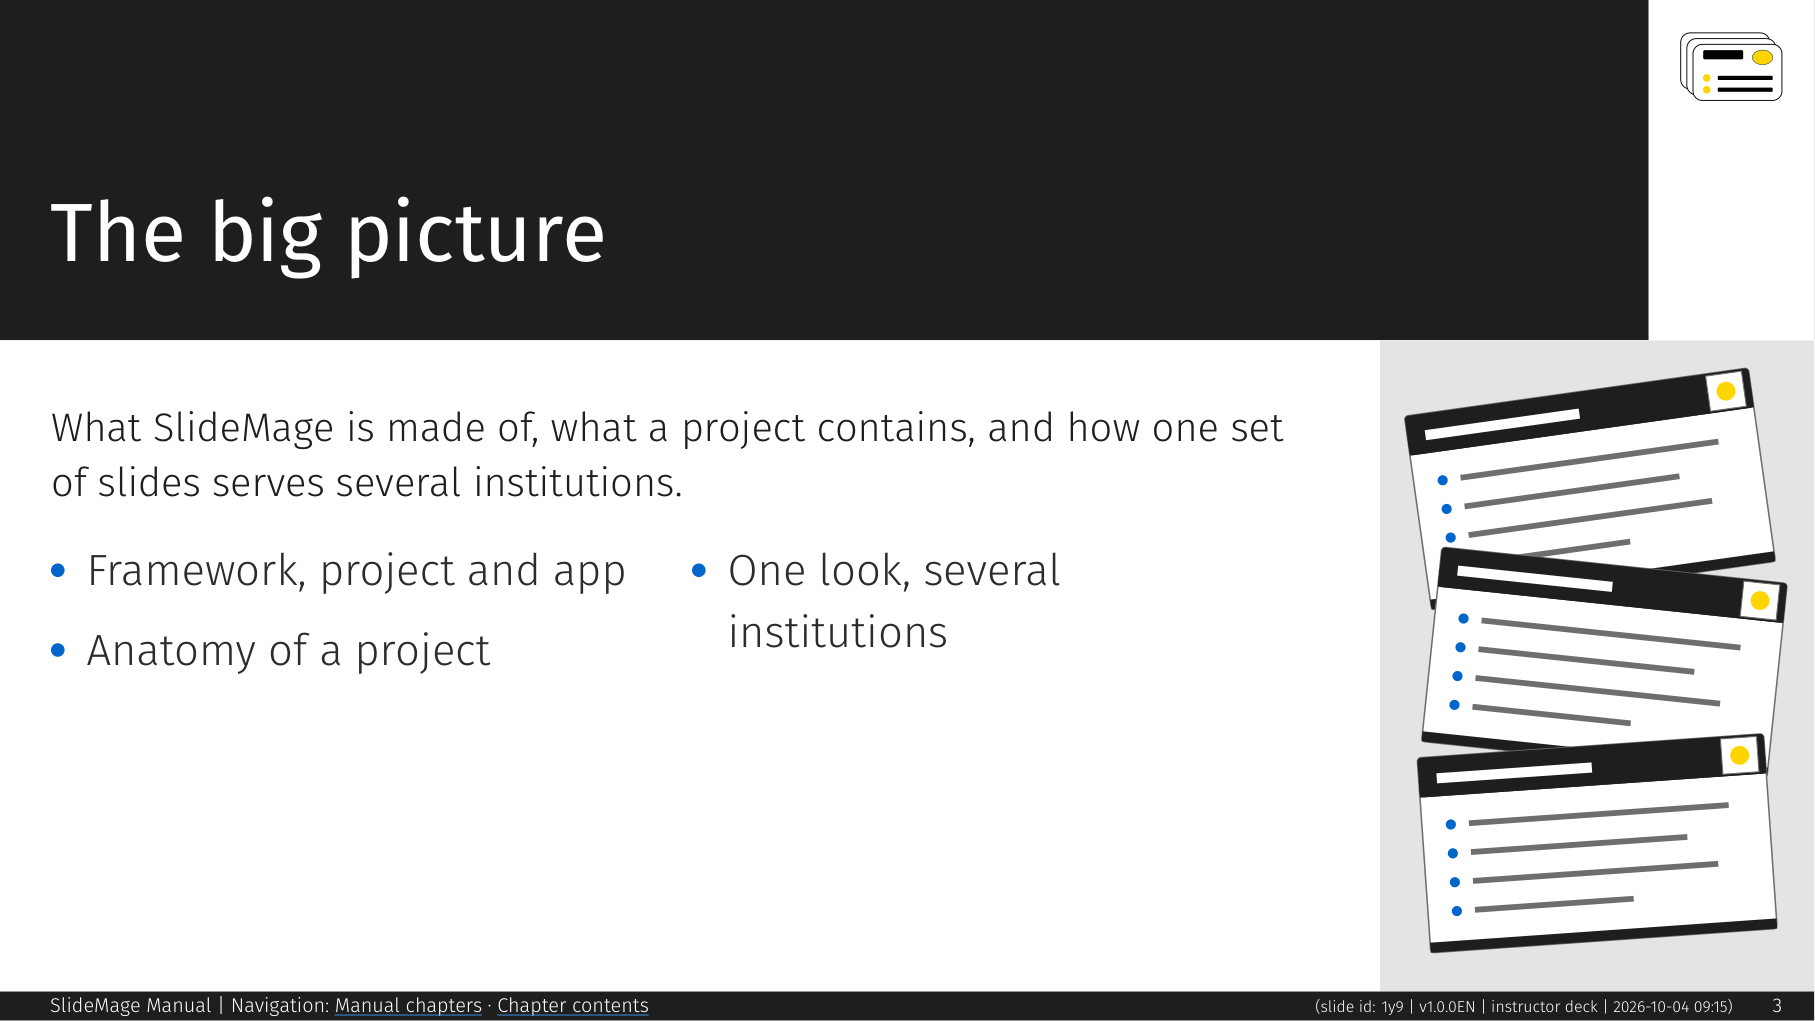
\includegraphics[width=86pt]{media/screenshot-slide-gallery-sectionframe.png}}{sectionframe} &
			\galleryitem{1y8}{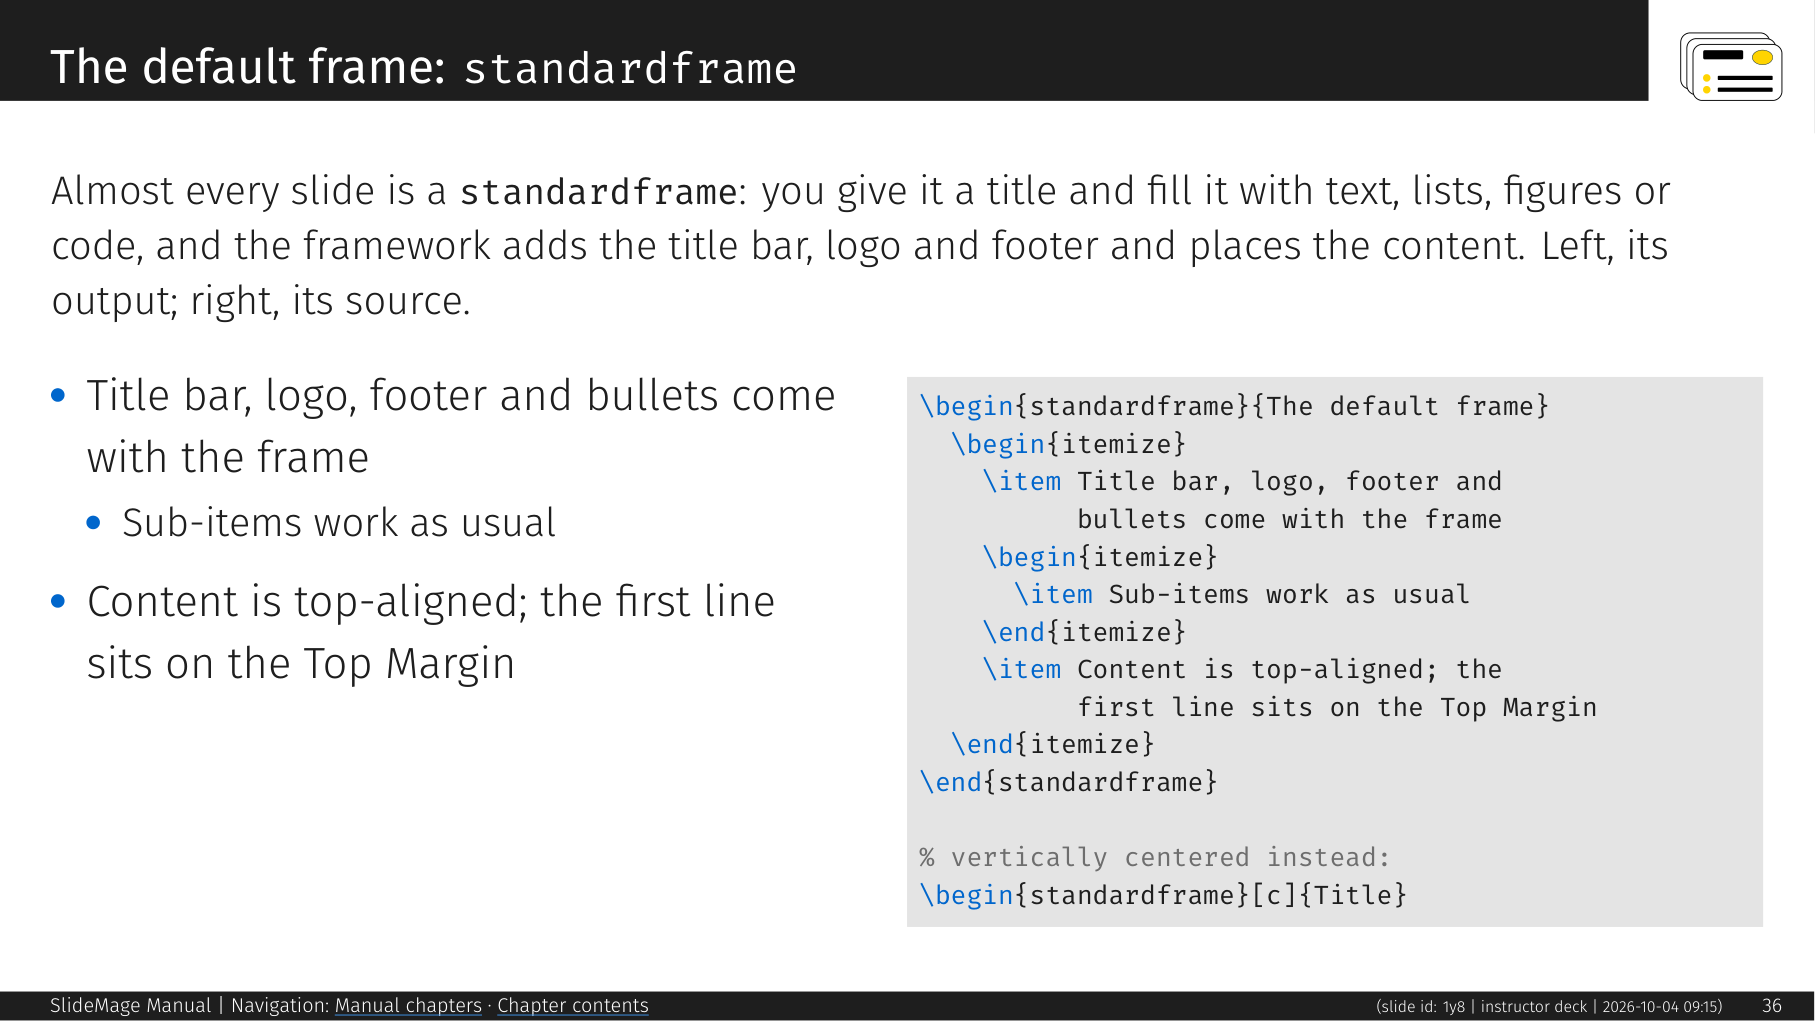
\includegraphics[width=86pt]{media/screenshot-slide-gallery-standardframe.png}}{standardframe} \\[1pt]
			\galleryitem{1i4}{
\includegraphics[width=86pt]{media/screenshot-slide-gallery-quoteframe.png}}{\textbackslash quoteframe} &
			\galleryitem{1vk}{
\includegraphics[width=86pt]{media/screenshot-slide-gallery-fullbleedframe.png}}{\textbackslash fullbleedframe} &
			\galleryitem{1rb}{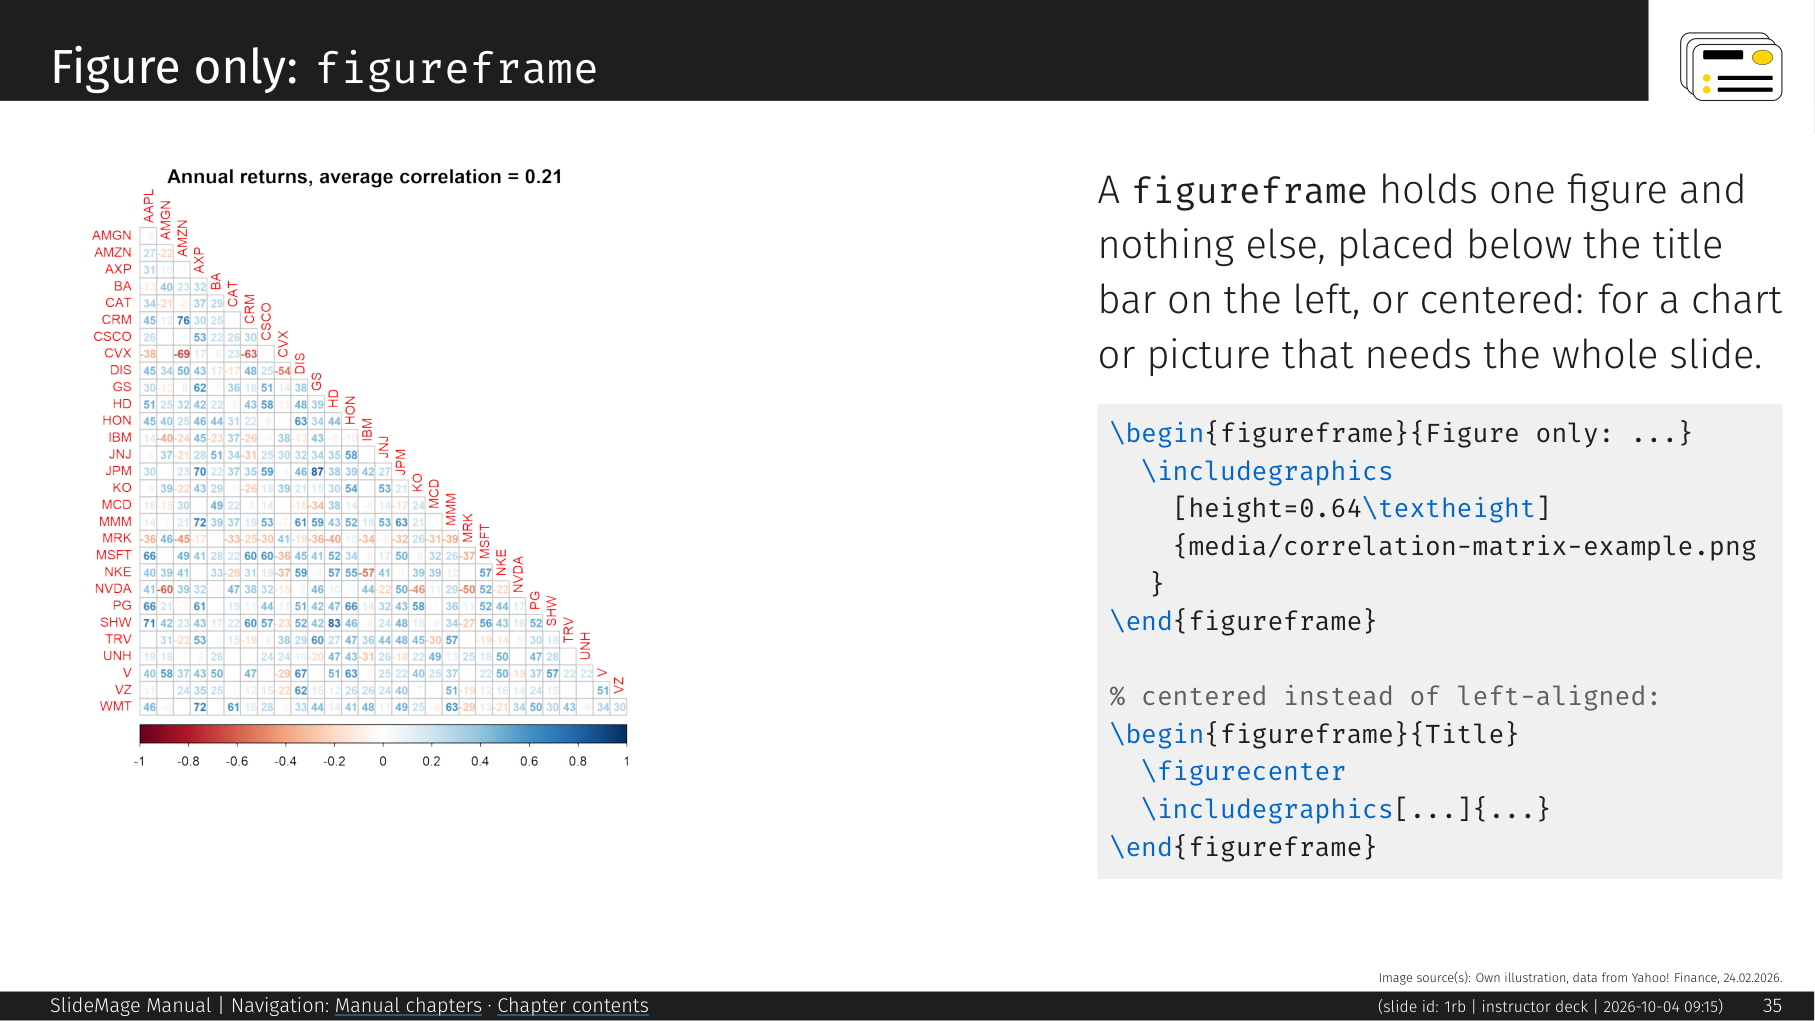
\includegraphics[width=86pt]{media/screenshot-slide-gallery-figureframe.png}}{figureframe} \\[1pt]
			\galleryitem{1vh}{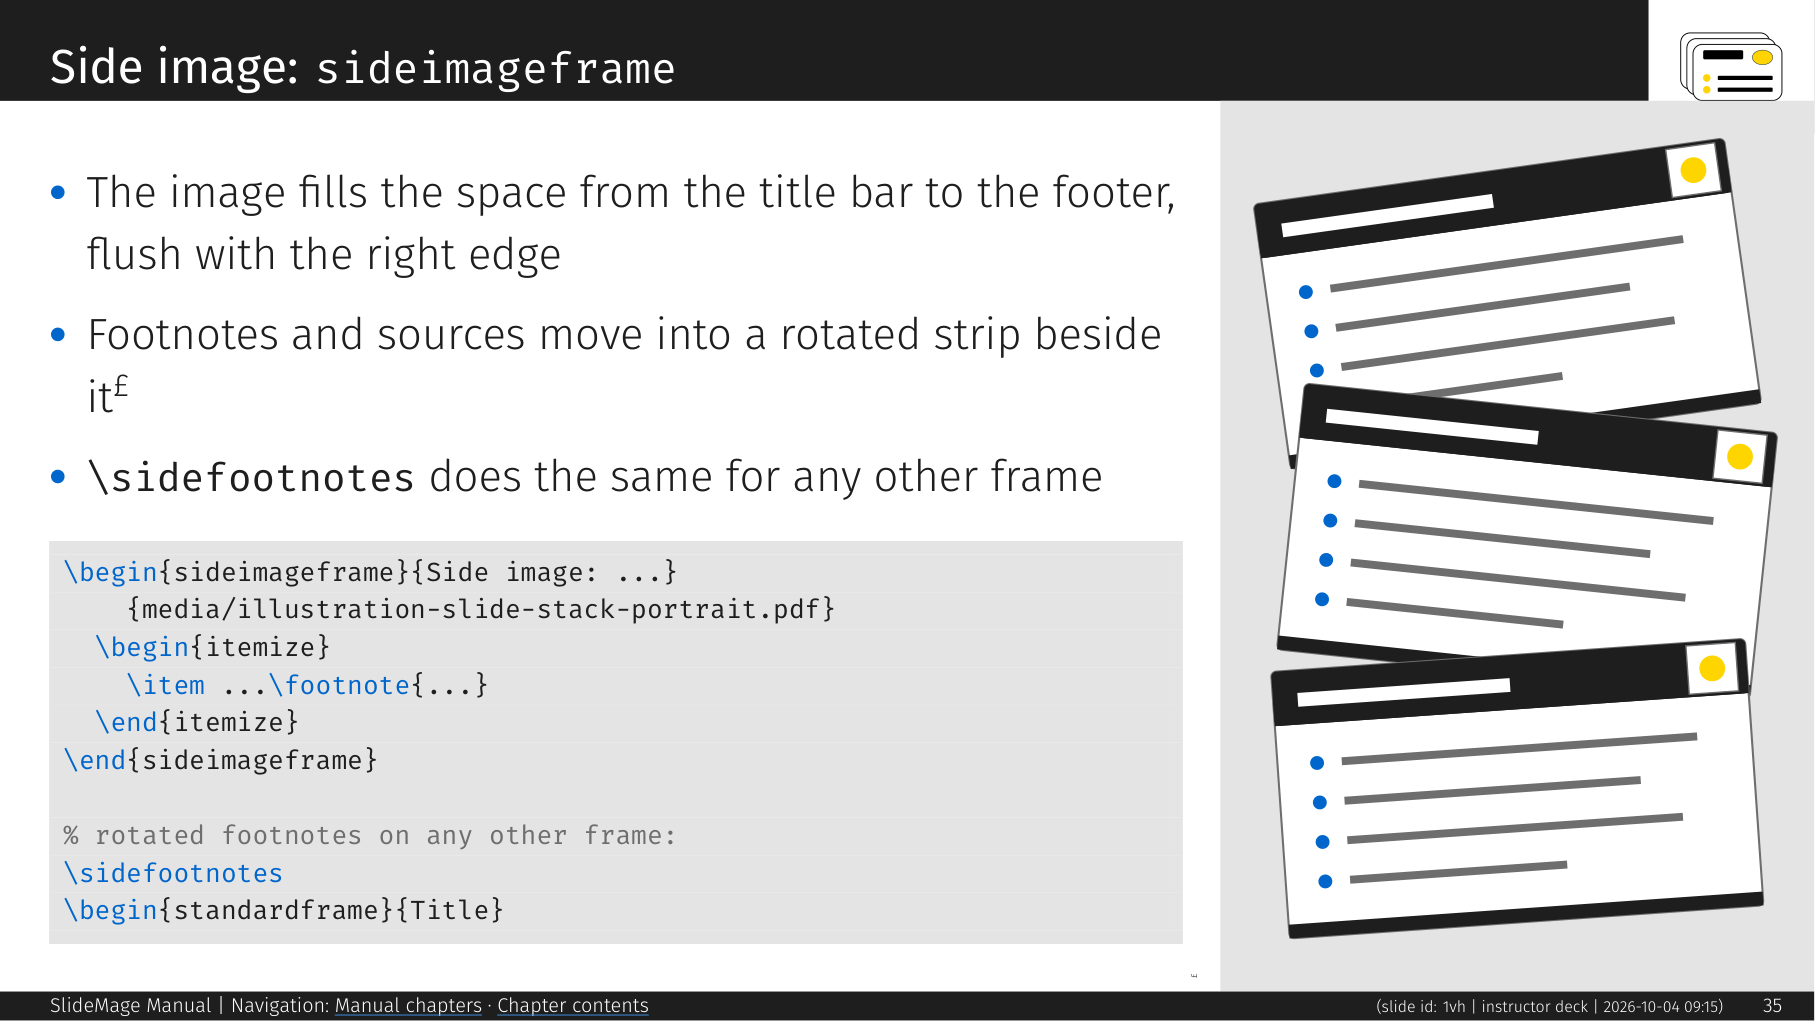
\includegraphics[width=86pt]{media/screenshot-slide-gallery-sideimageframe.png}}{sideimageframe} &
			\galleryitem{1mb}{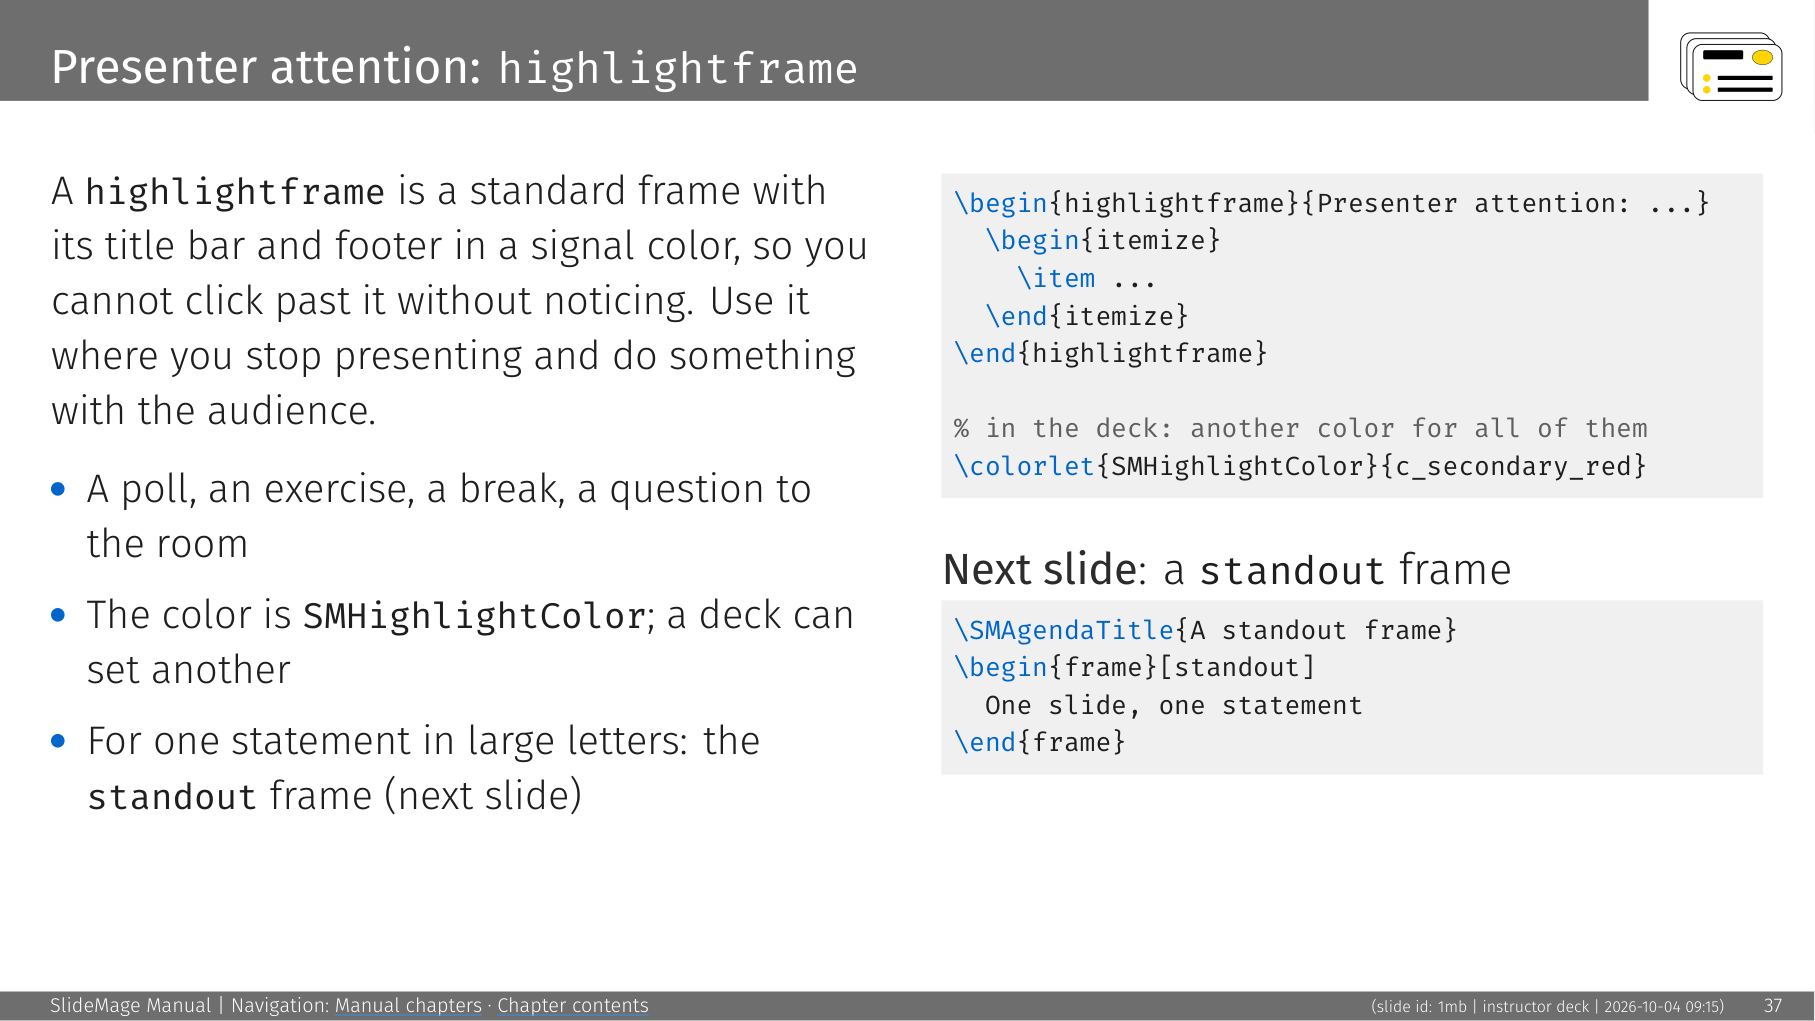
\includegraphics[width=86pt]{media/screenshot-slide-gallery-highlightframe.png}}{highlightframe} &
			\galleryitem{1xf}{
\includegraphics[width=86pt]{media/screenshot-slide-gallery-standout.png}}{[standout]}
		\end{tabular}
	\end{minipage}%
	\hfill
	\begin{minipage}[t]{0.31\linewidth}\vspace{0pt}
		\begin{itemize}
			\item Nine frame types, each with its own slide in this chapter
			\item Click one to jump there
			\item The footer's \emph{Chapter contents} brings you back
		\end{itemize}
		\medskip
		\hyperlink{1x7}{\beamerreturnbutton{Linking and navigating}}
	\end{minipage}
\end{standardframe}
